\documentclass[journal]{IEEEtran}
\usepackage{lmodern}
\usepackage{amsfonts}
%\usepackage{hyperref}

\usepackage{cite}
\ifCLASSINFOpdf
  \usepackage[pdftex]{graphicx}
  \graphicspath{{./img/}}
  \DeclareGraphicsExtensions{.pdf,.jpeg,.png}
\else
\fi
\usepackage{array}
\usepackage{url}
\hyphenation{op-tical net-works semi-conduc-tor av-er-age at-tribute}


\begin{document}
\title{Analysis of Genetic Algorithms Optimizing Topological Layout and Synaptic Weights }

\author{Taras~Mychaskiw~(4105797)~\textless{}tm07qx@brocku.ca\textgreater\\%
Evan~Verworn~(4582938)~\textless{}ev09qz@brocku.ca\textgreater% <-this % stops a space
}


\maketitle

\begin{abstract}
  The purpose of this experiment was to compare the results of training artificial neural networks
  through standard backpropation and using a genetic algorithm. The genetic algorithm altered both
  the structure and weights of the network to attempt to further encourage learning.
\end{abstract}

\IEEEpeerreviewmaketitle

\section{Introduction}
\IEEEPARstart{T}{his} experiment saught to compare the results of neural network learning by backpropation
versus using a genetic algorithm. The genetic algorithm would evolve the structure and synaptic weights
of the network simultaneously, attempting to optimize all the parameters. We found that the genetic algorithm
performed better overall on average, but may not have been worth the additional computation time.

\section{Background}
% I don't think we'd have to write much on this and GAs.
% I think about the same as a wikipedia summary.
  \subsection{Neural Networks}
  A high level description of a basic Neural Network is a single directional graph without
  cycles or reflexive edges. It is a mathematical model wherein given some number of inputs
  and some number of outputs, the outputs will react to the magnitude of the input values. A
  visualization is given in Figure \ref{fig:NeuralNetwork}.

\begin{figure}[here]%[!t]
  \centering
  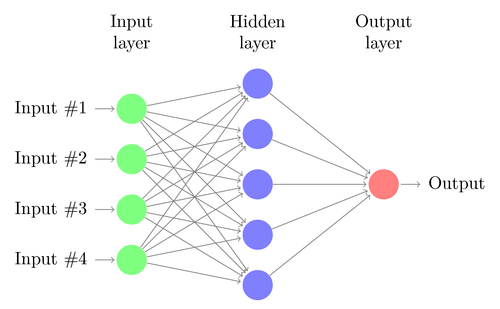
\includegraphics[width=3.4in]{neural-network}
  \caption{An example single hidden layer neural network.}
  \label{fig:NeuralNetwork}
\end{figure}

The output is \textit{trained} to the desired output through manipulating the weights in the
intermediate (hidden) and output layer edges.

\begin{figure}[here]
  \[  NodeOutput = \sum_{i=1}^{n} w_{i} x_{i} \]
  \caption{Where $n$ is the number of edges coming \textit{into} this node, $w$ is the weight
  associated with that edge and x is the output value produced by the predecessor node.}
  \label{fig:NodeOutput}
\end{figure}

A node calculates its output value by summing the output of all of its predecessors and multiplying
that output by a weight assigned to that edge, this value is then squashed to a number traditionally
between 0 and 1 by a Sigmoid function.

In the Figure \ref{fig:NeuralNetwork} there is only one hidden layer, but in our experiments we
are evolving a network that can have up to three hidden layers.

In this experiment, \texttt{brainjs} (written by Heather Arthur) was used for the backpropation learning.\cite{brain}

% Talk about backprop.
\subsubsection*{Learning}
A neural network learns by examples. Training examples are fed into the network, and the network changes
the synapse weights so that when training is complete, the network will produce the required results when
fed new problems it has not seen during training. The learning process is called \textit{Back-Propagation}.\cite{slides}

  \subsubsection*{Gradient Descent}
  Gradient descent is a common first order optimization algorithm. The is the reason we use a sigmoid
  activation function instead of the Heaviside function; the gradient of Heaviside is undefined at
  $x=0$. Gradient descent has it's basis in vector calculus. The gradient of a multi-variable function
  points in the direction of fastest growth of that function. The negative gradient then points in the
  direction where the function decreases the fastest. The function, in the case for neural networks,
  is the error of the system, $f(\omega_1,..,\omega_n)$, a function of all the weights of the network.
  The basic gradient descent weight update rule is
  \begin{equation}
    \vec{\omega} \leftarrow \vec{\omega} - \nu\vec{\nabla}\xi(\omega)
    \label{equ:grad}
  \end{equation}
  where $\vec{\omega}$ is the synapse weights, $\nu$ is the learning rate, and $\xi(\omega)$ is the error function.
  The error function value can be determined during the \textit{Back-Propagation} step, then one component
  of $\vec{\omega}$ is updated using Equation~\ref{equ:gradcomp}, where $g(\omega_i)$ is just the activation
  function of the neuron.\cite{3p71text}
  \begin{equation}
    \omega_i \leftarrow \omega_i - \nu\frac{\partial}{\partial\omega_i}g(\omega_i)
    \label{equ:gradcomp}
  \end{equation}

  \subsubsection*{Back-Propagation}
  A network is first initialized by setting all of the synapse weights to small random numbers, usually
  between $-1$ and $1$. A training example is fed into the network, and the output is calculated. Since
  each weight is a random number, the network output is completely different from the target output.
  The strategy is to calculate the error produced by each neuron. At the output layer, the error is simply
  $TargetOutput - ActualOutput$. According to the gradient descent equations, the error at the output layer is
  \begin{equation}
    err = \frac{\partial}{\partial\omega}g(x) \times (TargetOutput-ActualOutput)
    \label{equ:errorout}
  \end{equation}
  where $x$ is the value of the weighted sum.\\
  Propagating the error back, the error at a hidden neuron $j$ is
  \begin{equation}
    err_j = \frac{\partial}{\partial\omega}g(x) \times \left(\sum\limits_i \omega_i \cdot err_i\right)
    \label{equ:errorhidden}
  \end{equation}
  where $i$ is a neuron in the next layer.\\
  Finally, with all the error function values found, the weights of all the synapses in the network
  are updated using Equation~\ref{equ:grad}.\cite{pdf}

  \subsection{Genetic Algorithms}
  Genetic Algorithms or GAs are another mathematical model for finding an optimized solution
  in a large search space. This model is based off of Darwinian Evolution in that the best performing
  current solutions are bred together mixing genetic information from both parents into their
  children (known as a crossover operation). These children are then evaluated, just as their
  parents were, and subjugated to the same breeding rules.

  Like in biological evolution corruption of the genetic code can happen, this is a possibly
  destructive mutation that encourages diversity between parents. This mutation can provide new
  genetic code to the child that it might benefit from that it couldn't have received from the parents.
  %This sets this optimization technique apart from traditional hill climbers that don't introduce

  The difficulty of this search method is programically defining the layout of the genetic code
  (a Chromosome) and creating different mutation and crossover functions that hopefully it can benefit from.

\section{Methodology}
%Maybe pictures for each mutation/crossover?
This goal of this experiment is to use a GA to optimize a neural network and compare the result
to that of a vanilla neural network trained by back propagation. The following are the graph
operations that were chosen as the crossover and mutation functions.
  \subsection{Mutations}
  Mutations are possibly destructive operations that encourage diversity and explore the search
  space. All of these mutations where weighted the same and had the same chance of being used
  in all of the experiments.
    % Trying to keep all titles as "graph based" as possible.
    \subsubsection{Add Node}
      If the current graph allows for more nodes add one in the first possible hidden layer and
      connect it to any proceeding nodes behind it. For each new output edge from this node,
      randomize the weight associated with it. So while the node might be `fully connected' to
      all proceeding nodes, as the weight approaches 0 that edge effectively becomes disconnected.

      This function can only add nodes to the hidden layers of the neural networks. The input and
       output layers have a fixed amount of nodes that must exist, but can be disconnected.

    \subsubsection{Remove Node}
      This randomly selects a non-output node with connections and removes all outgoing
      connections. This function can disconnect input layer nodes. This could be considered
      beneficial to the network as `feature selection' and could remove data that could
      potentially add noise to the input layer, and then get propagated down the line.

    \subsubsection{Add Edge}
      This method selects a random edge and changes its value.

      If the edge does not exist it is created with a uniformly distributed `weight of connectivity'
      ranging from $ [0...1) $.
      If the edge does exist, a new value within the same range is given and the weight is overridden.

    \subsubsection{Remove Edge}
      Randomly selects a connected edge to remove. There is no restriction in what layer this can happen.
  %\subsubsection{Change Edge Weight}
  \subsection{Crossovers}
  Crossovers build off of existing solutions and exploit the genetic code we have found thus far to be useful.
    \subsubsection{Union}
    A union of all nodes and edges of the two graphs, if two edges exist on the two graphs then
    weights of both edges are averaged and this value becomes the new weight in the child.

    This is a crossover that can easily create bloat in the child that doesn't help it in any way.
    This child now has the superior genetic code of both parents with all of the unhelpful (malignant)
    mutations from both. \cite{lachlan} %ROBOTS IN DISGUISE

    \subsubsection{Intersection}
    The intersection function is a `clean-up' function, but can be very destructive if there
    is too much diversity between two parents. Just like in biological evolution if there is
    too much difference between the parents (different species) the child may not be as functional
    as each of the parents.

    When this type of crossover is selected, all edges and nodes that both parents share get
    passed onto the child. All other nodes/edges that are not shared by \textbf{both} parents
    is discarded.  \cite{lachlan}

    This function helps to reduce bloat that is created from the different mutations.

    \begin{figure}[!here]%[!t]
      \centering
      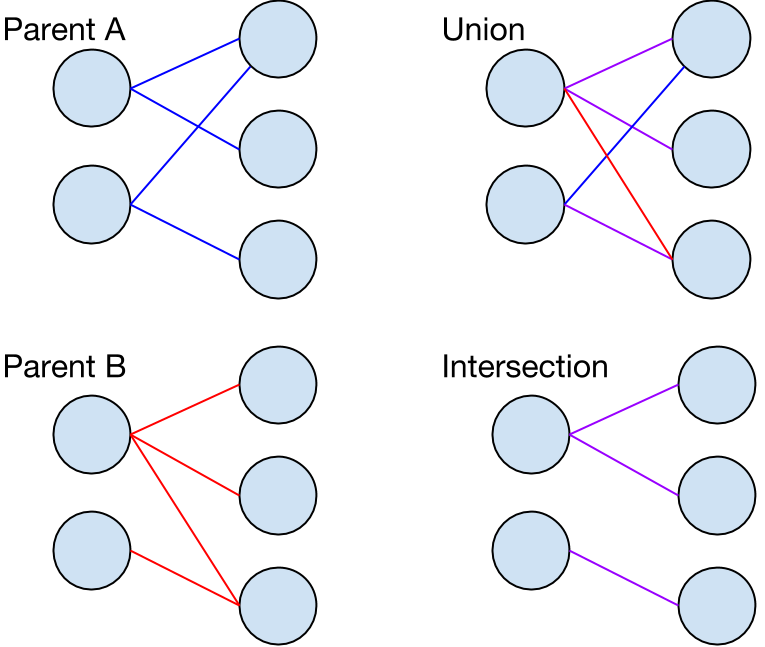
\includegraphics[width=3.4in]{ga_union_intersect}
      \caption{Example of union and intersection crossovers.}
      \label{fig:ga_union_intersect}
    \end{figure}

    \subsubsection{Roulette Union}
    An alteration to the standard union crossover. Instead of merging both parents into
    one child, a coin is flipped which decides which parent to take an edge from. If heads, then
    the edge from Parent A is copied exactly, else the edge from Parent B is copied.

    If both parents have a connection from node $ A \rightarrow B $ then there is a 100\% chance
    that the edge $A \rightarrow B$ exists. If one parent has a connection $A \rightarrow B$ and
    the other doesn't, then there is a 50/50 chance of the child receiving the link or not,
    compared to inheriting all edges like the previous mentioned union.

    This is done for all aspects of both parents, if both parents have the same aspect it will
    for sure show up in the child. This is more how biological evolution works wherein the
    Chromosome is built from a random selection of a little of Parent A and a little of Parent B.
    
  \subsection{Tournament}
  From a population the `best' individuals must be chosen to pass their genetic code onto future generations. 
  The method through which these are chosen is through a tournament selection.
  
  After all the individuals have been given a fitness, the best $n$ individuals are taken from
  the generation to be bred against each other. Using the following function.
  
\begin{verbatim}
for i in new_population
  if(mutation)
    i := best_individuals[random()].mutate()
  else if(crossover)
    first := best_individuals[random()]
    second:= best_individuals[random()]
    while first == second
      second := best_individuals[random()]
    i = first.crossover(second)
\end{verbatim} 

% maybe this should go infront of methodology.
\section{Experiments}
  The purpose of this project is to compare results of vanilla backpropation to the results of
  a Genetic Algorithm applied to optimizing a neural network's weights and topography.

  Traditionally a comparison like this only focuses on the GA optimizing the weights \textbf{or}
  the topography of the neural net. We have attempted to do both simultaneously. We found the
  results from the first problem to be inconclusive and desided to run more experiments on a second
  problem.

  The first problem is in need of feature reduction with it's many inputs and few possible outputs.

  The second problem is a noisy data problem with many key variables it must compare for the final
  result.

  \subsection{Connect 4}
   This dataset contains all legal 8-ply positions in the game of
   connect-4 in which neither player has won yet, and in which the next
   move is not forced.

   The input is the full state of the board (who is in each position) and the expected output
   is either `win', 'loss' or 'draw' for the `first player'.

   This experiment's description could be simplified to creating a neural network as the heuristic
   function of a connect-4 board.

  \subsection{Quality of Wines}
  Two datasets were created, using red and white wine samples.
  The inputs include objective tests (e.g. PH values) and the output is based on sensory data
  (median of at least 3 evaluations made by wine experts). Each expert graded the wine quality
  between 0 (very bad) and 10 (very excellent).

  These datasets were then merged together. The input layer contains
  "fixed acidity", "volatile acidity", "citric acid", "residual sugar", "chlorides",
  "free sulphur dioxide", "total sulphur dioxide", "density", "pH", "sulphates" and "alcohol"
  for each of the wines.

  The expected output is a single value between 0 and 10.\cite{wine}

  \begin{table}[here]
    \renewcommand{\arraystretch}{1.3}
    \caption{Genetic Algorithm Run Parameters}
    \label{E2}
    \centering
    \begin{tabular}{r|cccc}
  Experiment      & 1     & 2     & 3     & 4 \\
  Generations     & 20    & 70    & 100   & 100 \\
  Population      & 200   & 200   & 200   & 100 \\
  Crossover       & 0.8   & 0.8   & 0.8   & 0.8 \\
  Mutation        & 0.2   & 0.2   & 0.2   & 0.2 \\
  Tournament Size & 50    & 50    & 50    & 50 \\
  Data Type       & C4    & W     & W     & W \\
  Data Size       & 18000 & 6000  & 6000  & 1000 \\
  Runs            & 36    & 72    & 48    & 24 \\
    \end{tabular} \\
  \textit{Where `C4' and `W' are the `Connect4 Data Set' and `Wine Data Set' respectively.}
   \end{table}

  \begin{table}[here]
    \renewcommand{\arraystretch}{1.3}
    \caption{Backpropagation Parameters}
    \label{E2}
    \centering
    \begin{tabular}{r|ccc}
  Experiment      & 1     & 2     & 3     \\
  Epochs          & 1000  & 1000  & 1000  \\
  Data Type       & C4    & W     & W     \\
  Data Size       & 6000  & 2000  & 2000  \\
  Runs            & 30    & 30    & 30    \\
    \end{tabular} \\
  \textit{Where `C4' and `W' are the `Connect4 Data Set' and `Wine Data Set' respectively.}
   \end{table}

\section{Analysis}
  \subsection{Connect 4}
    \subsubsection*{$Run_{GA}$ 1) Union/Intersect}
      \begin{figure}[here]%[!t]
        \centering
        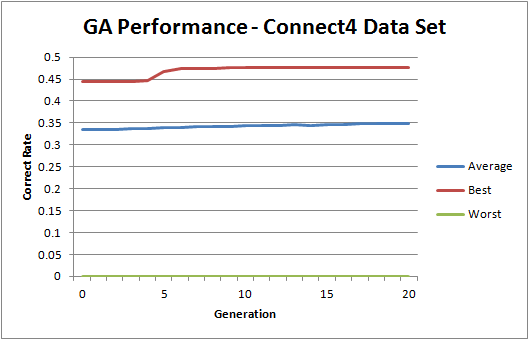
\includegraphics[width=3.4in]{connect4_performance_new}
        \caption{An example single hidden layer neural network.}
        \label{fig:connect4_performance_new}
      \end{figure}
      From Figure~\ref{fig:connect4_performance_new} and Figure~\ref{fig:brain_connect4}
    we can see that the Connect 4 problem is computationally hard to learn, and may not
    be worth it when each generation takes 32 minutes long.

      Unfortunately when looking at Figure~\ref{fig:connect4_performace_new} it can be seen
    that very little learning occurs over the course of the experiment. Random guessing
    which should (for this problem) result in a fitness of 0.33. This is what the average
    population starts at. The average population at the end of the experiment is only ~0.35
    leading me to speculate that all `learning' that occured was a result of random search.
    This is further supported by the `best' in all runs having a fitness of 0.44 in generation 0 and only
    increasing to 0.47 by generation 20.

    With these findings it can be concluded with the standard Union and Crossover functions
    mentioned above would not be benifitial to encourage learning for this problem.

    \subsubsection*{$Run_{NN}$ 1) Vanilla Backprop}
      \begin{figure}[here]%[!t]
        \centering
        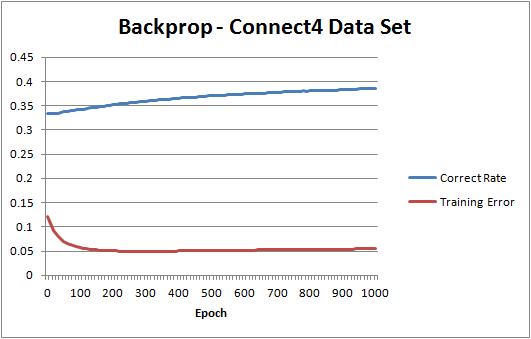
\includegraphics[width=3.4in]{brain_connect4}
        \caption{An example single hidden layer neural network.}
        \label{fig:brain_connect4}
      \end{figure}
    When looking at Figure~\ref{fig:brain_connect4} it can be seen that vanilla backprop
    at generation 0 is simply guessing the answer, at the end of the experiment it can be
    seen that the backprop did learn increasing its' correctness on the testing set to 0.37.
    More than the average of the GA in the previous experiment, but clearly not very successful.
    
    While vanilla backprop performed worst overall compared to the best of the GA, it can be argued that
    backprop was the `winner' in this competition because it was able to \textbf{learn}. Compared to
    the GA, which found its best in generation 0 through random search.
    
  \subsection{Wine Quality}
    \subsubsection*{$Run_{GA}$ 2) Union/Intersect}
      \begin{figure}[here]%[!t]
        \centering
        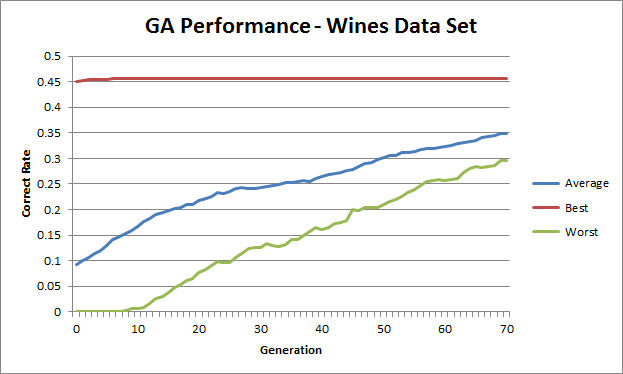
\includegraphics[width=3.4in]{wine_performance_new}
        \caption{An example single hidden layer neural network.}
        \label{fig:wine_performace_new}
      \end{figure}
      Unfortunately the learning curve is very similar to the first experiment. The GA over 6 generaions
      quickly found the most successful solution through random search, which isn't surprising when considering
      that over 6 generations each with a population of 200 over 72 runs is a solution set of 86400 random permutations.
      
    \subsubsection*{$Run_{GA}$ 3) Uniform}
      \begin{figure}[here]%[!t]
        \centering
        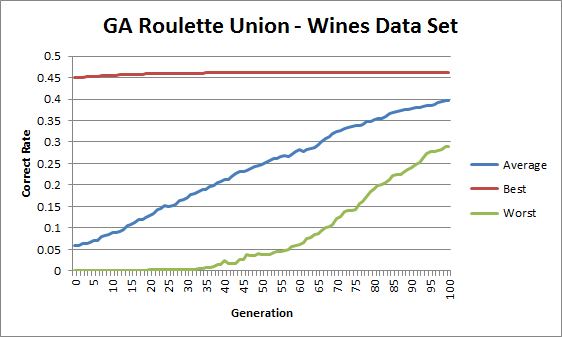
\includegraphics[width=3.4in]{wine_uniform}
        \caption{An example single hidden layer neural network.}
        \label{fig:wine_uniform}
      \end{figure}

    \subsubsection*{$Run_{GA}$ 4) Change}
      \begin{figure}[here]%[!t]
        \centering
        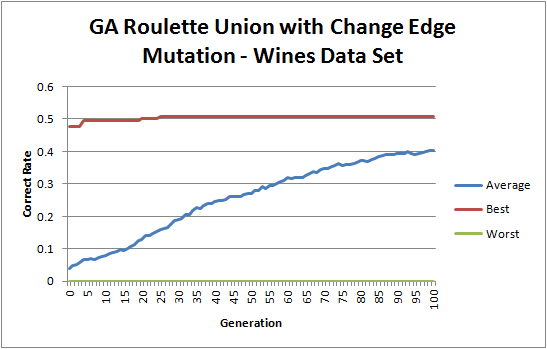
\includegraphics[width=3.4in]{wine_change_edge}
        \caption{An example single hidden layer neural network.}
        \label{fig:wine_change_edge}
      \end{figure}

    \subsubsection{$Run_{NN}$ 2) Vanilla Backprop}
      \begin{figure}[here]%[!t]
        \centering
        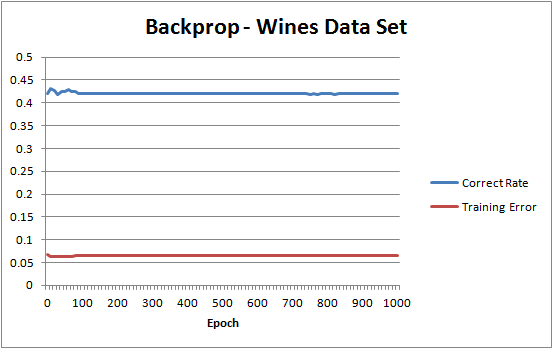
\includegraphics[width=3.4in]{brain_wine}
        \caption{An example single hidden layer neural network.}
        \label{fig:brain_wine}
      \end{figure}
    Clearly, Figure~\ref{fig:brain_wine} shows that no learning took place. All that can be concluded from this
    is \textit{perhaps} that the inputs for this particular data set do not correlate with the quality of the wine.

\section{Conclusion}
Things could have done better.

We believe this is due to crossovers used.

Blah-de-Blah.


% references section


\bibliographystyle{IEEEtran}
\begin{thebibliography}{1}

\bibitem{lachlan}
Lachlan Plant, Graph Theory Consultant

\bibitem{brain}
"brainjs" Retrieved April 2013 from
http://harthur.github.io/brain/

\bibitem{wine}
  P. Cortez, A. Cerdeira, F. Almeida, T. Matos and J. Reis.
  Modeling wine preferences by data mining from physicochemical properties.
  In Decision Support Systems, Elsevier, 47(4):547-553. ISSN: 0167-9236.

\bibitem{pdf}
"The Backpropagation Algorithm" Retrieved February 2013 from
http://www4.rgu.ac.uk/files/chapter3 - bp.pdf

\bibitem{slides}
Ombuki-Berman, B. "COSC 4P80 Lecture Slides" Brock University, Winter 2012/13

\bibitem{3p71text}
Russell, S. J., and P. Norvig. "Artificial Intelligence, A Modern Approach." Pearson College Div, 2010.

\end{thebibliography}

% Can be used to pull up biographies so that the bottom of the last one
% is flush with the other column.
%\enlargethispage{-5in}

% that's all folks
\end{document}
